\label{anexo}
\subsection{Output de la Consultas Propuestas por el Enunciado}
Estos outputs pueden encontrarse en el notebook \texttt{propuestas\_del\_enunciado.ipynb}. 
\subsubsection{Consulta 1}
\textbf{Output de la Validación}

\label{anexo:output_validacion_consulta1}
\begin{lstlisting}[style=console]
Filas totales en dataset orders: 4700000
Filas con estado no nulos: 4277862
Filas con estado nulo: 422138
Todas las filas que tienen estado nulo, tienen direccion de facturacion indefinida? Si
\end{lstlisting}

\textbf{Filtro de Estados}

\label{anexo:output_filtro_estados}
\begin{lstlisting}[language=Python]
not_states_filter = ~(
    orders["state"].str.contains("AA")   # Military Americas
    | orders["state"].str.contains("AE") # Military Europe
    | orders["state"].str.contains("AP") # Military Pacific
    | orders["state"].str.contains("FM") # Federated States of Micronesia
    | orders["state"].str.contains("MH") # Marshall Islands
    | orders["state"].str.contains("MP") # Northern Mariana Islands
    | orders["state"].str.contains("PW") # Palau
    | orders["state"].str.contains("GU") # Guam
    | orders["state"].str.contains("VI") # U.S. Virgin Islands
    | orders["state"].str.contains("AS") # American Samoa
    | orders["state"].str.contains("PR") # Puerto Rico
    | orders["state"].str.contains("DC") # District of Columbia
    | orders["state"].isna()             # Nulos
)
print("Cantidad de estados: ", orders.loc[not_states_filter]["state"].unique().size)
print("Estados considerados: ", orders.loc[not_states_filter]["state"].unique())
\end{lstlisting}
\begin{lstlisting}[style=console, aboveskip=0pt]
Cantidad de estados:  50
Estados considerados:  ['ND' 'NJ' 'MN' 'WI' 'OH' 'NV' 'MA' 'AZ' 'MO' 'VT' 'MI' 'NY' 'NM' 'PA'
 'WY' 'NE' 'WV' 'KY' 'WA' 'TX' 'OK' 'ME' 'KS' 'IN' 'FL' 'MD' 'MS' 'AL'
 'MT' 'ID' 'NC' 'AK' 'SD' 'NH' 'SC' 'CT' 'CA' 'CO' 'GA' 'IA' 'VA' 'OR'
 'DE' 'LA' 'UT' 'AR' 'IL' 'TN' 'RI' 'HI']
\end{lstlisting}

\textbf{Formateo de los Resultados}
El archivo json utilizado con los nombres de estado puede encontrarse junto con el código fuente del proyecto.
\label{anexo:output_formateo_resultados}
\begin{lstlisting}[language=Python, xleftmargin=70pt, xrightmargin=70pt]
import json
with open("state_names.json", "r") as f:
    state_names = json.load(f)

quantity_of_orders_with_discounts_by_state["Nombre del Estado"] = 
    quantity_of_orders_with_discounts_by_state["state"].map(state_names)

quantity_of_orders_with_discounts_by_state.rename(
    columns={
        "order_id": "Cantidad de Ordenes con Descuento",
        "state": "Codigo de Estado"
        }, inplace=True
    )
\end{lstlisting}

\subsubsection{Consulta 2}

\textbf{Códigos postales con 5 órdenes `Refunded'}

\label{anexo:output_codigos_postales_refunded}
\begin{lstlisting}[language=Python, xleftmargin=35pt, xrightmargin=35pt]
print("\nCodigos postales con 5 ordenes 'Refunded':")
print(amount_refunded_orders_by_zipcode.loc[amount_refunded_orders_by_zipcode["count"] == 5])
\end{lstlisting}
\begin{lstlisting}[style=console, aboveskip=0pt, xleftmargin=145pt, xrightmargin=145pt]
Codigos postales con 5 ordenes 'Refunded':
   zip_code  count
1     65247      5
2     38151      5
3      9045      5
4     14396      5
5     73291      5
6     91623      5
\end{lstlisting}

\textbf{Otros nombres que aparecen en órdenes `Refunded'}

\label{anexo:nombres_mas_comunes}
\begin{lstlisting}[language=Python, xleftmargin=105pt, xrightmargin=105pt]
print("\nOtros nombres que aparecen una sola vez:")
print(most_common_names.loc[most_common_names == 1].head(7))
\end{lstlisting}
\begin{lstlisting}[style=console, aboveskip=0pt, xleftmargin=145pt, xrightmargin=145pt]
Otros nombres que aparecen una sola vez:
first_name
ROBERT     1
CYNTHIA    1
JAY        1
MARIA      1
KAREN      1
CARLA      1
WILLIAM    1
\end{lstlisting}

\subsubsection{Consulta 3}
\textbf{Gráficos Heatmap resultantes}
\label{anexo:consulta3_heatmap}

\begin{figure}[H]
    \centering
    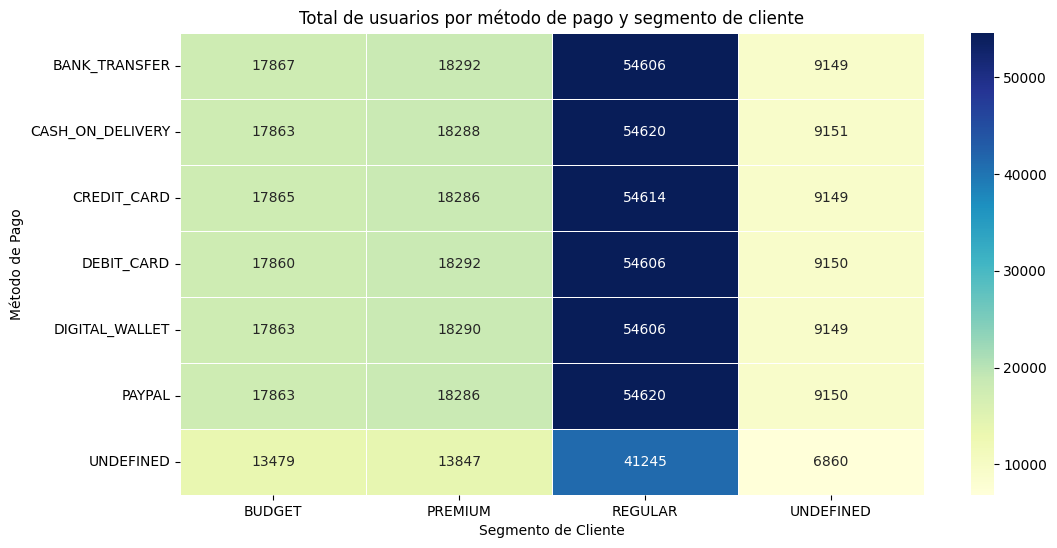
\includegraphics[width=0.8\textwidth]{imagenes/consulta3_heatmap1.png}
\end{figure}

\begin{figure}[H]
    \centering
    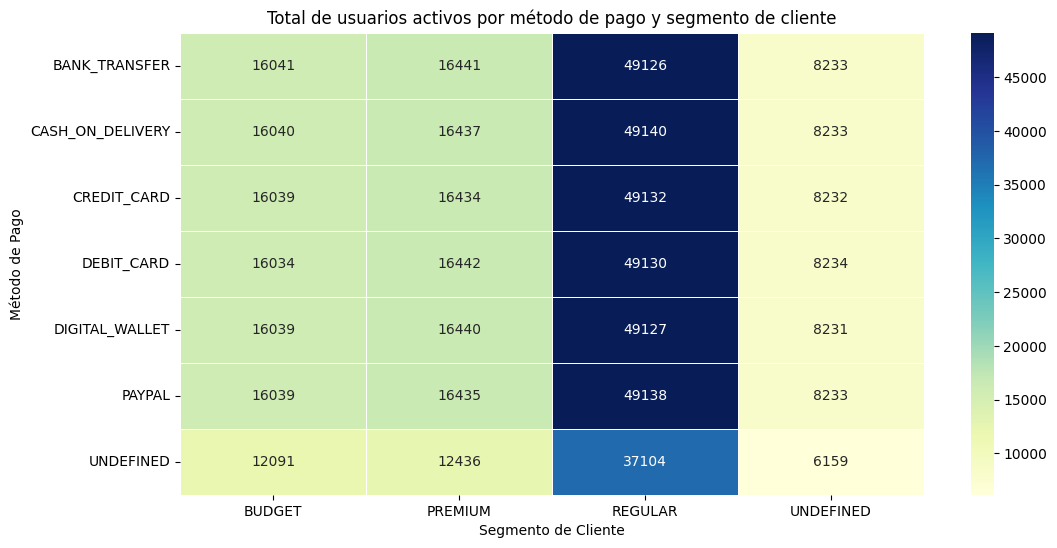
\includegraphics[width=0.8\textwidth]{imagenes/consulta3_heatmap2.png}
\end{figure}

\begin{figure}[H]
    \centering
    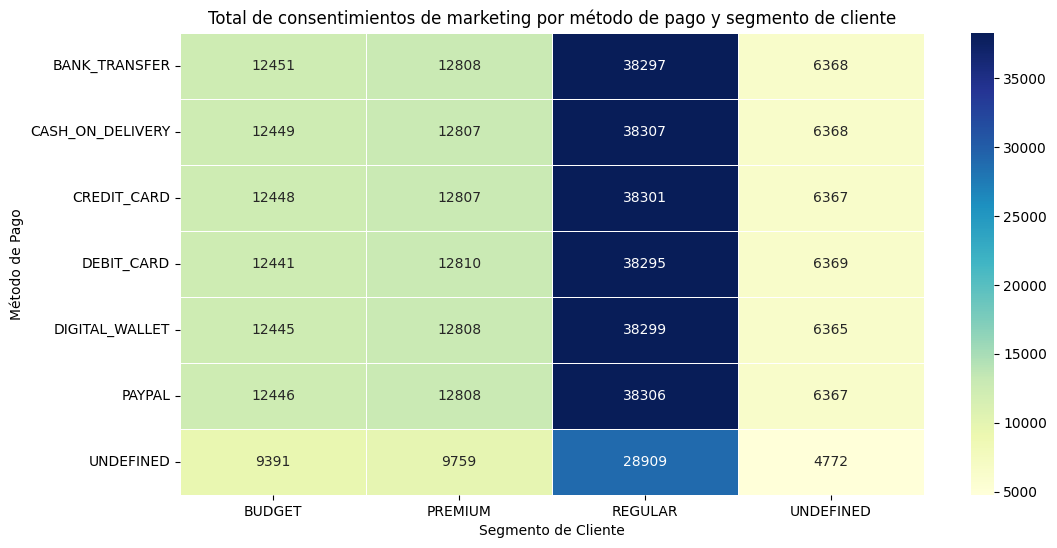
\includegraphics[width=0.8\textwidth]{imagenes/consulta3_heatmap3.png}
\end{figure}

\begin{figure}[H]
    \centering
    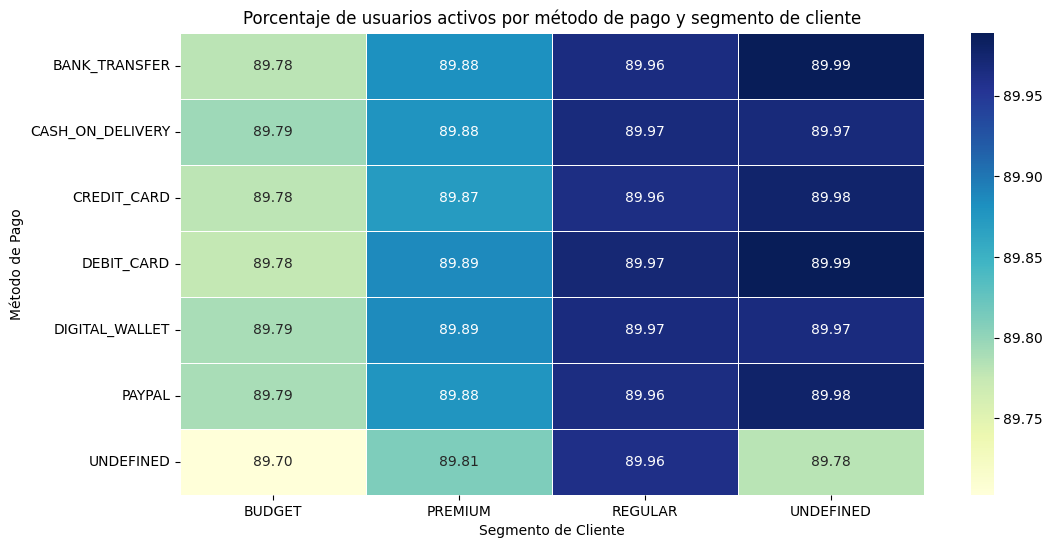
\includegraphics[width=0.8\textwidth]{imagenes/consulta3_heatmap4.png}
\end{figure}

\begin{figure}[H]
    \centering
    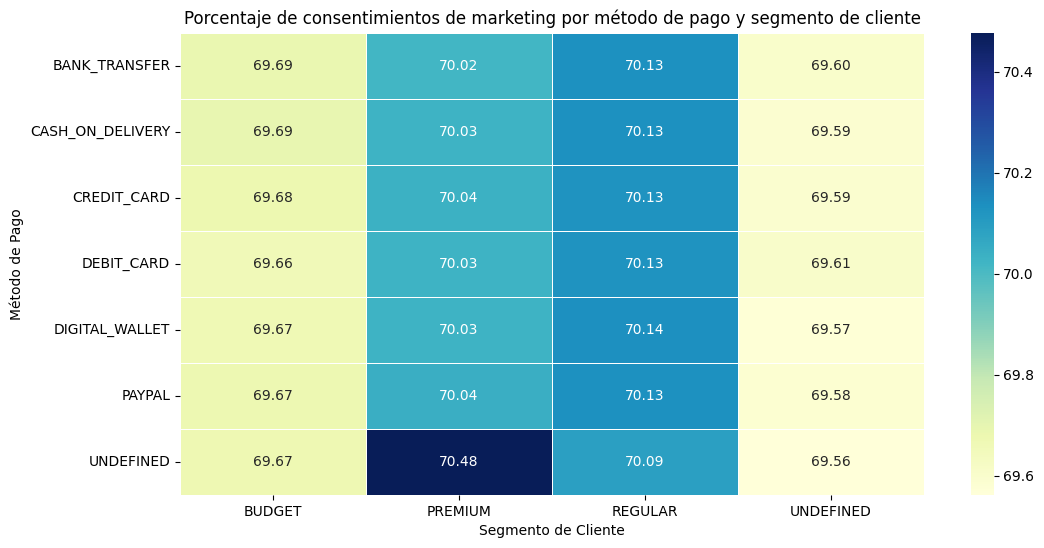
\includegraphics[width=0.8\textwidth]{imagenes/consulta3_heatmap5.png}
\end{figure}